\documentclass{beamer}
\usepackage[utf8]{inputenc}
\usepackage[francais]{babel}
\usepackage[T1]{fontenc}
\usepackage{lmodern}
\usepackage{ifpdf}
\usepackage{graphicx}
\usepackage{geometry}
\usepackage{color}
\usepackage{pdfpages}
\usepackage{hyperref}

%\usetheme{Berlin}
\usetheme{Warsaw}

% ------------------------------------------------------------------------------
% TITLE
% ------------------------------------------------------------------------------

\title{Zigful-Meyer}
\subtitle{Un test partiel de Fugl-Meyer fait par Kinect}
\author{William Dyce \and Geoffrey Melia}
\institute
{
  Université Montpellier 2
}
\date{22 Février 2013}


% ------------------------------------------------------------------------------
% TITLE
% ------------------------------------------------------------------------------

\begin{document}

\begin{frame}[plain]
  \titlepage
\end{frame}
%-----------------------------------------------------------------------------
% PART 0 - INTRODUCTION
% ------------------------------------------------------------------------------

\begin{figure}[h!]
\centering
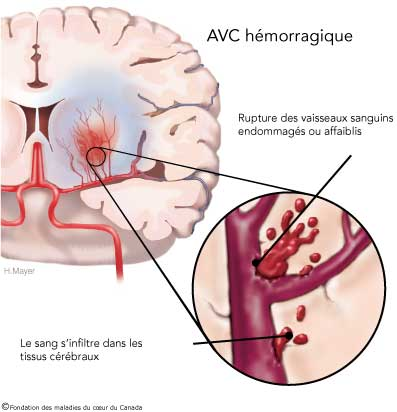
\includegraphics[width=0.5\linewidth]{images/avc}
\caption{Accident Vasculaire Cérébrale (AVC).}
\end{figure}

Les accidents vasculaires cérébraux (AVC) peuvent être la cause d'hémiplégie chez les personnes qui en sont victimes. La paralysie peut affecter une ou plusieurs parties du corps, jusqu'à être totale si la face, le tronc et les membres supérieurs et inférieurs sont paralysés. \\
La récupération des fonctions motrices, de la parole ou de la compréhension dépendent pour beaucoup de l'âge du patient et de son atteinte au niveau du cerveau.
    \section{Problématique}
Il existe de nombreux tests et échelles pour évaluer les capacités sensorimotrices de patients hémiplégiques \footnote{voir l'Analyse de la littérature \textit{Evaluation of the disabilities of hemiplegic patients [M.-C. Gellez-Leman et al.]}}. Cependant, les médecins se retrouvent souvent confrontés au problème de la précision des mesures lors des test. Si la question ne se pose pas pour les tests dits \textit{fonctionnels} (ex : le patient arrive t-il à se servir un verre d'eau?), des mesures d'angles et de positions se révèlent souvent nécessaires pour valider ou non la réussite d'un test par le patient.
\\Or, il existe peu d'outils pour réaliser ces mesures, et ceux-ci ne font pas l'unanimité. Pour la mesure d'angle entre les membres du patient (pli de l'épaule, du coude, etc.), le goniomètre se révèle être l'outil le plus utilisé, mais probablement par défaut (cf \ref{lapeyronie} ). On lui reprochera en effet d'être: 
\begin{itemize}
  \item {intrusif :} Il doit être en contact direct avec le patient, pouvant fausser la mesure ou aider/gêner le patient.
  \item {imprécis :} L'épaisseur de peau et de graisse ne permet pas d'évaluer correctement l'angle formé par les os.
  \item {inutilisé :} Des médecins pourtant équipés vont préférer juger à l'œil, pour un meilleur ratio temps/précision.
\end{itemize}

    \subsubsection{Le test de Fugl-Meyer}
Cette imprécision des mesures devient dès lors gênante lorsque c'est un test non pas fonctionnel, mais de déficience qui est considéré comme le "Gold Standard" dans le domaine : le score de Fugl Meyer [\ref{fugl_meyer}]. En effet, celui-ci consiste à évaluer les mouvements du patient lors de la réalisation de gestes très précis, incluant des mouvements "éliminatoires", qu'il faut donc être capable de mesurer.  
  
  L'idée s'est alors posée d'utiliser un autre moyen de mesure, moins intrusif, pour la réalisation de test de Fugl Meyer, largement utilisé dans le milieu de la réhabilitation, et de réfléchir aux possibilités d'enrichissement de celui-ci.
\newpage
    \section{Présentation du projet}
    
      \subsection{Étude de terrain} \label{etude_terrain}
    Le projet est avant tout une étude de faisabilité. Nous essayerons de voir
    à quel point nous pouvions procéder, avec un capteur de profondeur (en
    l'occurrence la Microsoft Kinect) et des bibliothèques et outils couramment 
    disponibles, à un test complet ou partiel de Fugl-Meyer.
    
    Nous étudierons donc d'une part les technologies disponibles pour la Kinect,
    et d'autre ce qu'est le test de Fugl-Meyer et quelles sont les 
    problématiques associées.
    
    \subsection{Prototype}
    Nous élaborerons ensuite une preuve de concept, c'est à dire un 
    prototype proposant au patient en cours de réhabilitation un test partiel 
    de Fugl-Meyer. Les points importants à considérer pour un tel prototype 
    sont~:
    \subsubsection{Automatisation et objectivité}
    Le système doit pouvoir procéder à une évaluation, de manière non-intrusive 
    et sans intervention externe, de ce qui se trouve devant lui. Il doit donc 
    proposer une série de notes objectives qui correspondent aux performances du 
    patient.
    \subsubsection{Aspect ludique~: "gamification"}
    La "gamification" est le processus qui consiste à ajouter des éléments 
    souvent associés au domaine du jeu (d'où le nom), comme des barres de
    progression ou des défis à relever, à une activité non-ludique. L'idée est 
    de favoriser l'implication et la motivation des participants. 
    Notons qu'il ne s'agit pas nécessairement de faire de l'activité en soi un 
    jeu.
    \subsubsection{Retour d'information continue et granulaire}
    La "granularité" d'un retour est le nombre d'options possibles. 
    Chaque exercice du Fugl-Meyer, par exemple, est noté sur trois points. Nous 
    aimerions proposer une alternative plus nuancée.
    L'argument pour le retour d'information rejoint celui de la "gamification"~:
    la notion de "sens" dans un jeu, au moins d'après Salen et Zimmerman, est 
    directement liée à la richesse de ce retour.


\begin{frame}
\tableofcontents[hideallsubsections]
\end{frame}

% -
% ------------------------------------------------------------------------------
% PART I - MEDICAL BACKGROUND
% ------------------------------------------------------------------------------

\section{Aspect médical}

\begin{frame}
\tableofcontents[currentsection, hideothersubsections]
\end{frame}


\subsection{Pré-requis}
\begin{frame}{Pré-requis}
	\begin{block}{Projet multidisciplinaire}
		\begin{itemize}
			\item Acquérir les connaissances médicales de base  \pause
			\item Comprendre les enjeux et le contexte médico-social  \pause
			\item Analyser quels peuvent être les besoins
		\end{itemize}			
	\end{block}  \pause
		\begin{block}{Étude de terrain}
		\begin{itemize}
			\item Recherche et études documentaires  \pause
			\item Premières suppositions   \pause
			\item Rencontrer patient et professionnels  \pause
			\item Confronter les idées
		\end{itemize}			
	\end{block}
\end{frame}

\subsection{Fugl-Meyer assessment}
\begin{frame}{Fugl-Meyer assessment}
	\begin{block}{Définition}
Mesure de la déficience motrice et sensorielle des membres supérieurs et inférieurs.
	\end{block}  \pause
	\begin{block}{Description}
Constitue un ensemble d'exercices dont chaque mouvement est évalué selon 1 ou plusieurs critères, permettant une évaluation de la sensibilité, du tonus, de la force et de la motricité du patient à travers l'analyse de son score.
	\end{block}
\end{frame}

\begin{frame}{Fugl-Meyer assessment}
	\begin{block}{Fonctionnement}
		Découpage permettant d'obtenir 3 sous-scores : 
		\begin{itemize}
			\item membre supérieur : 33 items, cotés 0 à 66
			\item membre inférieur : 17 items, cotés 0 à 34
			\item équilibre : 7 items, cotés 0 à 14
		\end{itemize}
	\end{block}  \pause
	\begin{block}{Précision}
		Décomposition de  la partie membre supérieur en 2 sections : 
		\begin{itemize}
			\item score distal \footnote{partie d’un membre la plus éloignée de la base de celui-ci} 
			\item score proximal\footnote{partie du corps proche de la racine d’un membre}
		\end{itemize}
	\end{block}	
\end{frame}

\begin{frame}{Fugl-Meyer assessment}
	\begin{figure}
	\centering
	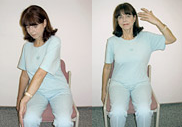
\includegraphics[width=6cm]{../images/fuglmeyer_example.png}
	\caption{Exemple d’un exercice du membre supérieur du test de Fugl-Meyer}
	\end{figure}
\end{frame}

\subsection{L'avis des professionnels}
\begin{frame}{L'avis des professionnels}
L'échelle sensorimotrice de Fugl Meyer :
	\begin{exampleblock}{Avantages}
			\begin{itemize}
			\item Constitue le "Gold Standard"  \pause
			\item Très utilisée en recherche et dans la littérature 
		\end{itemize}  \pause
	\end{exampleblock}
	\begin{alertblock}{Critiques}
			\begin{itemize}
			\item Variabilités des résultats : imprécision des mesures, subjectivité de la notation  \pause
			\item Faible amplitude de mesure : effet "plateau", pas représentatif des progrès   \pause
			\item Test de déficiences et non fonctionnel
		\end{itemize}
	\end{alertblock}	
\end{frame}

% ------------------------------------------------------------------------------
% PART II - KINECT BACKGROUND
% ------------------------------------------------------------------------------

\section{Le Kinect}

\begin{frame}
\tableofcontents[currentsection, hideothersubsections]
\end{frame}

\subsection{Matériel}
\begin{frame}{Matériel}
\vbox to 1.0\textheight
{
\begin{block}{Spécifications techniques~\cite{kinect_msdn}\cite{wiki_kinect}}
  \begin{minipage}[t]{0.49\linewidth}
    \begin{itemize}
    %\item<1-> \emph{caméra couleur}\only<1->{~:
    \item \emph{caméra couleur}
    \begin{itemize}
    \item 1280x960 à 12Hz,
    \item 640x480 à 30Hz.
    \end{itemize}%}
    %\item<2-> \emph{étalage de 4 microphones},
    \item \emph{étalage de 4 microphones}
    \end{itemize}
  \end{minipage} 
  \begin{minipage}[t]{0.49\linewidth}
    \begin{itemize}
    %\item<3-> \emph{capteur de profondeur}\only<3->{~:
    \item \emph{capteur de profondeur}
    \begin{itemize}
    640x480 à 30Hz.
    \end{itemize}%}
    %\item<4-> 
    \item \emph{moteur},
    %\item<4-> 
    \item \emph{accéléromètres}.
    \end{itemize}
  \end{minipage}
\end{block}
  \begin{center}
    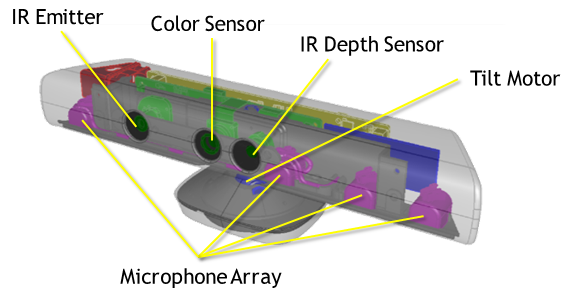
\includegraphics[height=0.4\textheight]{../images/kinect_specs}
  \end{center}
  \vfill
}
\end{frame}

%\subsection{Pilotes}
%\begin{frame}{Pilotes}

%\vbox to 1.0\textheight
%{
%  \begin{itemize}
%  \item sortie du Kinect le 4 Novembre 2010,
%  \begin{itemize}
%  \item Adafruit offre \$3000 de prime~\cite{adafruit_bounty}.
  
%  \only<1>
%  {
%  \vfill
%  \begin{center}
%  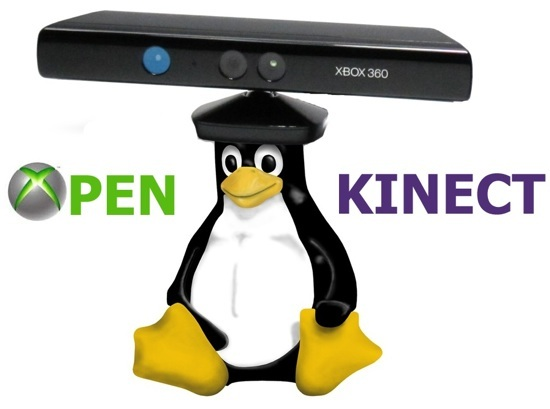
\includegraphics[width=0.65\textheight]{../images/kinect_tux}
%  \end{center}
%  }
  
%  \end{itemize}
%    \item<2-> \textbf{Libfreenect} sort le 10 Novembre 2010~\cite{adafruit_winner},
    
%    \only<2>
%    {
%    \vfill
%    \begin{center}
%    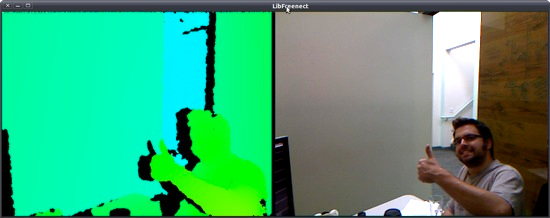
\includegraphics[width=0.9\linewidth]{../images/hector}
%    \end{center}
%    }
    
%    \item<3-> \textbf{CL-NUI} sort le 19 Novembre 2010~\cite{clnui},
    
%    \only<3>
%    {
%    \vfill
%    \begin{center}
%    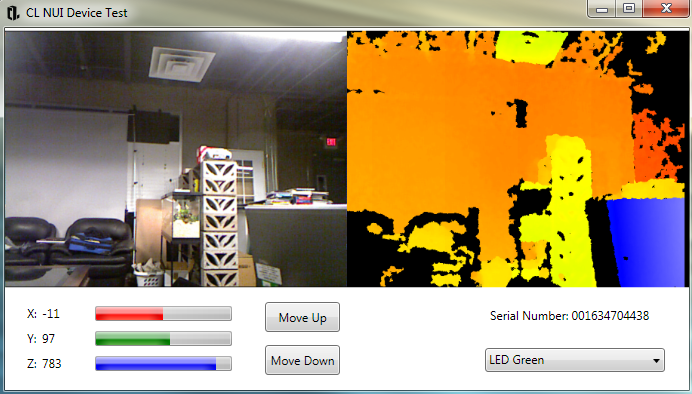
\includegraphics[width=0.6\linewidth]{../images/clnui}
%    \end{center}
%    }
    
%    \item<4-> \textbf{Kinect for Windows}~:
%    \only<4->
%  {
%    \begin{itemize}
%      \item en bêta le 16 Mai 2011,
%      \item version complète le 1 Février 2012,
%    \end{itemize}
%  }
%  \item<5-> \textbf{OpenNI SDK}.
  
%  \only<5>
%  {
%  \begin{minipage}{0.49\linewidth}
%    \centering
%    
\includegraphics[width=0.9\linewidth]{../images/openni_logo}
%  \end{minipage}
%  \begin{minipage}{0.49\linewidth}
%    \centering
%    
\includegraphics[width=0.9\linewidth]{../images/primesense_logo}
%  \end{minipage}
%  }
  
%  \end{itemize}
%\vfill
%}
%\end{frame}

\subsection{Pilotes}
\begin{frame}{Pilotes}
\begin{center}
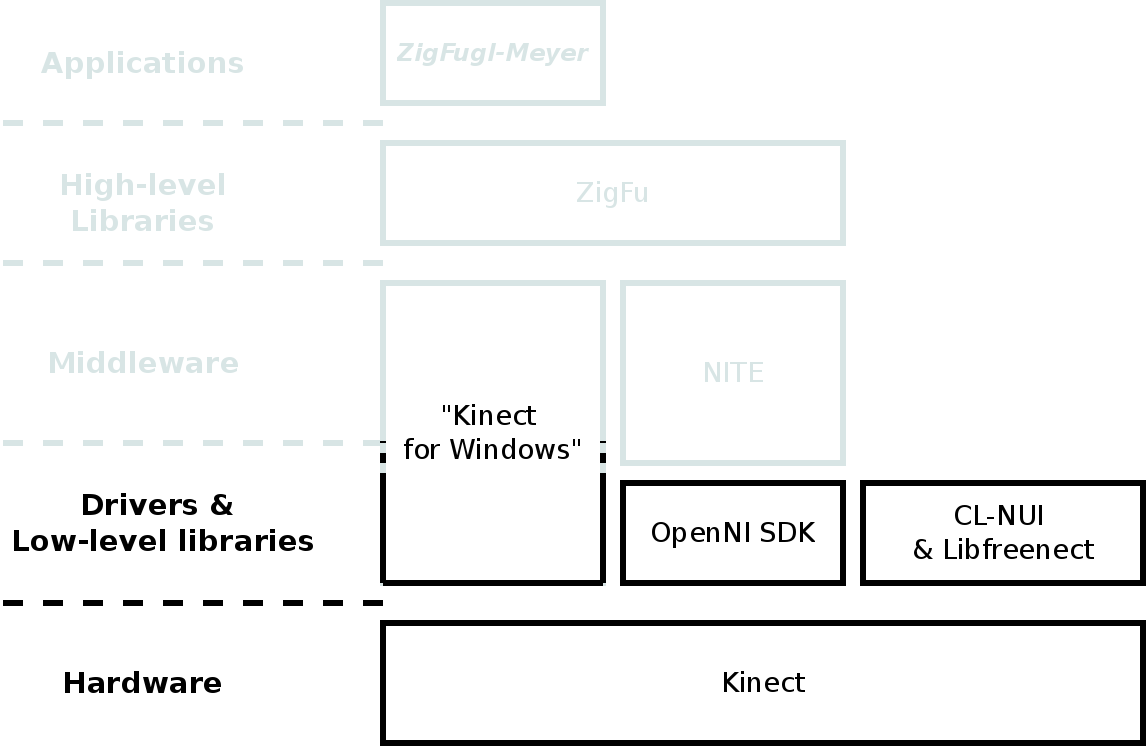
\includegraphics[width=0.9\linewidth]{../images/technology_overview_1}
\end{center}
\end{frame}

\subsection{Middleware}
\begin{frame}{Middleware}
\begin{center}
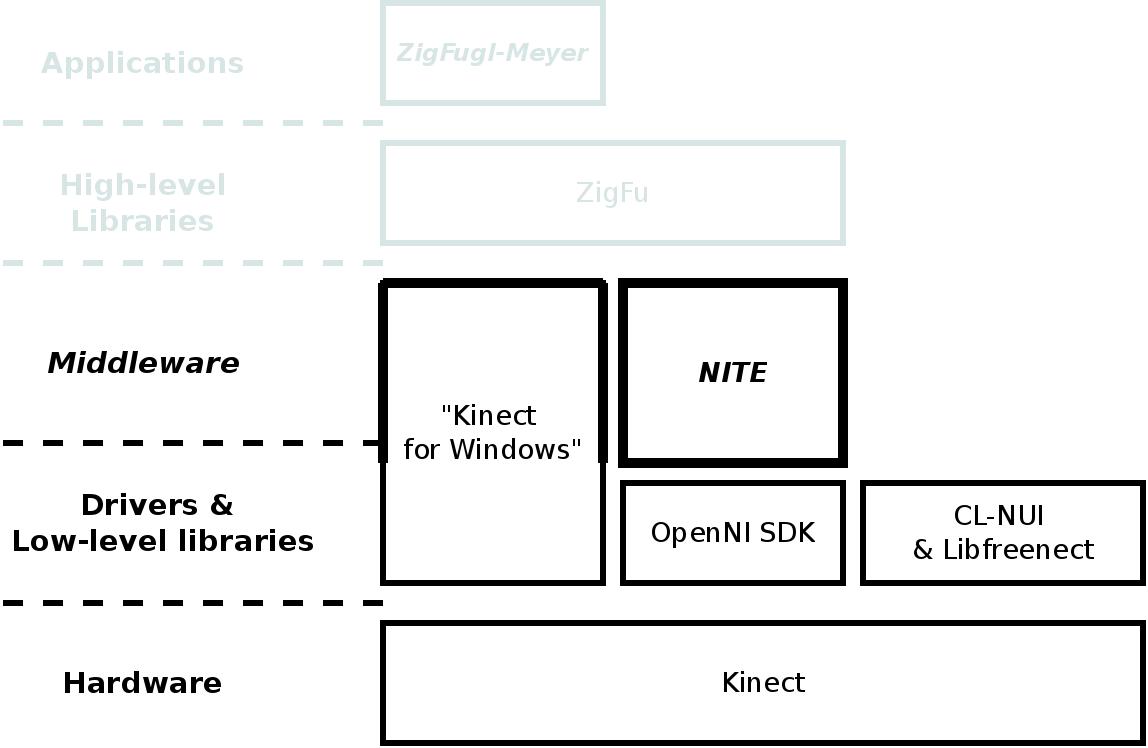
\includegraphics[width=0.9\linewidth]{../images/technology_overview_2}
\end{center}
\end{frame}

\begin{frame}{Kinect for Windows~\cite{microsoft_vs_openni_2}}
\vbox to 1.0\textheight
{
\begin{itemize}
  \item<1-> Prédictif, gère mieux l'occlusion partielle (apprentissage)
                ~\cite{how_you_become_the_controller}~\cite{shotton2011},
  \only<1>
  {
    \vfill
    \begin{center}
    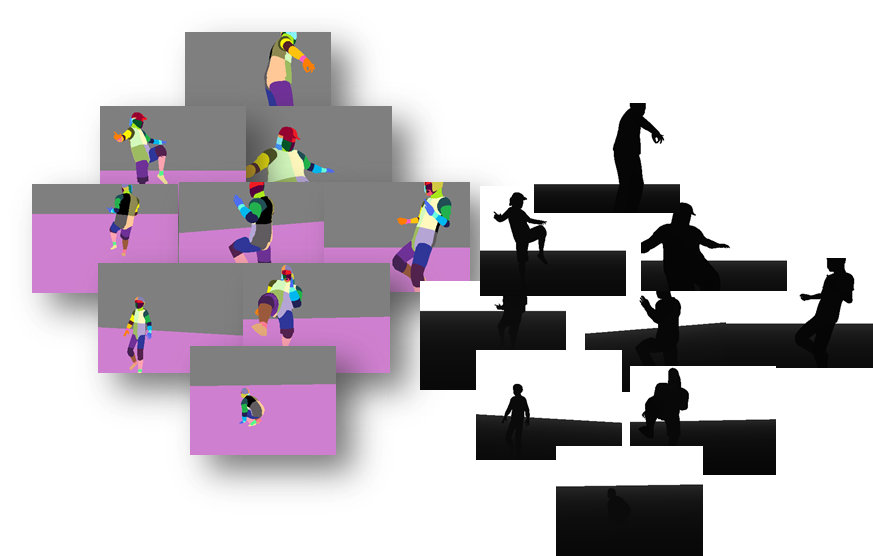
\includegraphics[width=0.7\linewidth]{../images/kinect_learning}
    \end{center}
  }
  \item<2-> Détection et suivi faciale,
  \only<2>
  {
    \vfill
    \begin{center}
    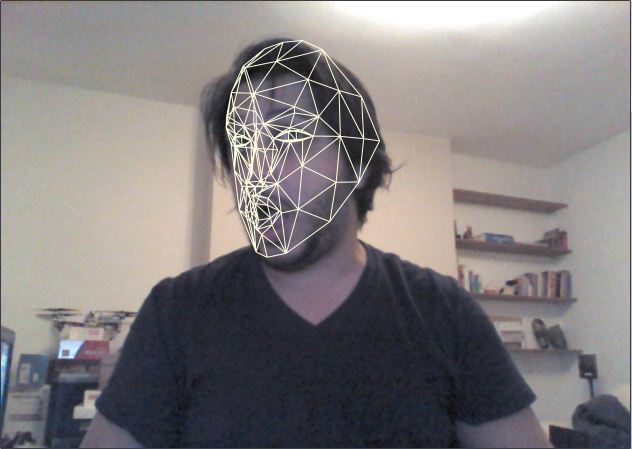
\includegraphics[width=0.5\linewidth]{../images/kinect_face_track}
    \end{center}
  }
  \item<3-> ``Kinect Fusion"~\cite{newcombe2011}~\cite{izadi2011},
  \only<3>
  {
    \vfill
    \begin{center}
    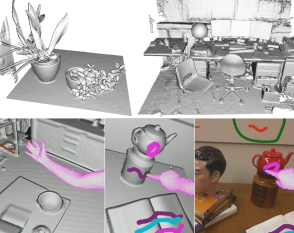
\includegraphics[width=0.4\linewidth]{../images/kinect_fusion}
    \end{center}
  }

\end{itemize}
\vfill
}
\end{frame}

\begin{frame}{OpenNI et NITE~\cite{microsoft_vs_openni}}
\vbox to 1.0\textheight
{
  \emph{OpenNI}
  \begin{itemize}
    \item<1-> Multiplateforme (Linux, Mac OS X),
    \item<2-> Standard ouvert~: middlewares alternatifs tiers,
    \only<2>
    {
      \vfill
      \begin{center}
      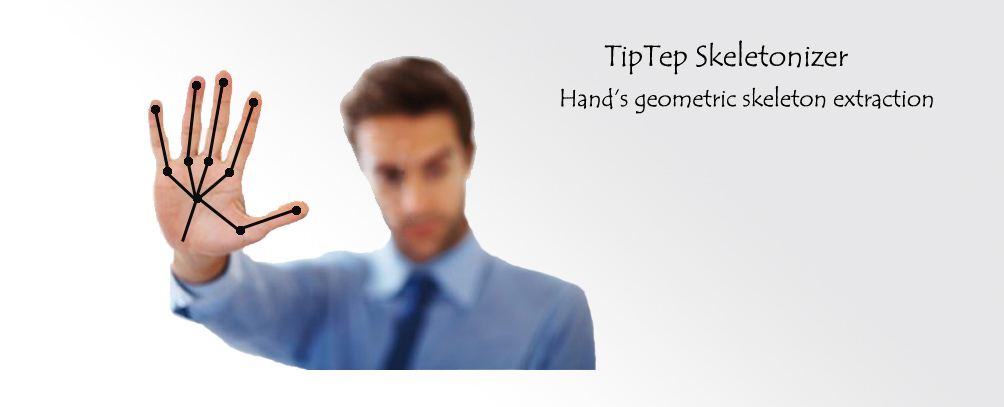
\includegraphics[width=0.8\linewidth]{../images/tiptep}
      \end{center}
    }
  \end{itemize}
  
  \only<3->
  {
  \emph{NITE}
  \begin{itemize}
    \item<3-> Moins de resources consommées,
    \item<4-> Moins de faux positives,
    \item<5-> Détection et suivie des \og{}gestures\fg{}.
  \end{itemize}
  }
\vfill
}
\end{frame}

\subsection{High-level libraries}
\begin{frame}{High-level libraries}
\begin{center}
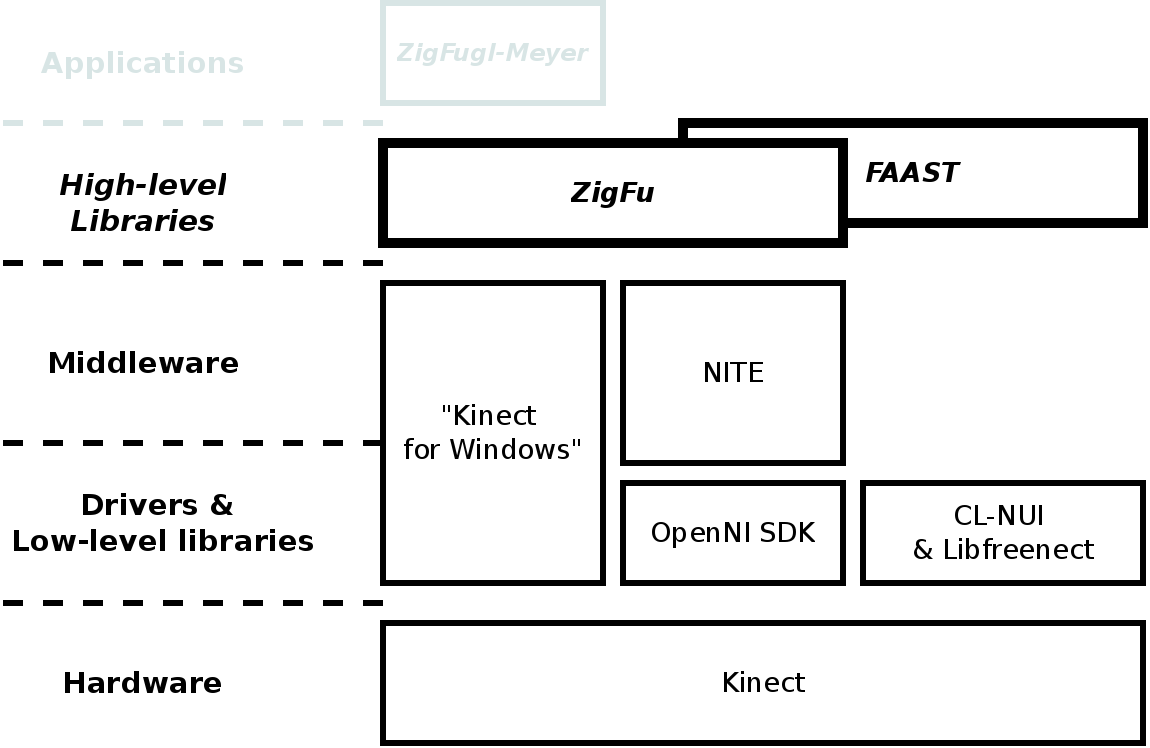
\includegraphics[width=0.9\linewidth]{../images/technology_overview_3}
\end{center}
\end{frame}

\subsection{Zigfu}
\begin{frame}{Zigfu}
\begin{block}{Features~\cite{zigfu_video}}
  \begin{itemize}
  \item Installation facile, 
  \item Bindings HTML 5, Unity 3D (et Flash bientôt),
  \item Lissage prédictif ($30 \rightarrow 60Hz$), 
  \item Cinématique inverse (simulation physique),
  \item Éléments GUI (boutons, listes, curseurs).
  \end{itemize}
\end{block}
\begin{center}

\includegraphics[width=0.2\linewidth]{../images/zigfu_logo}
\end{center}
\end{frame}

\subsection{Résumé}
\begin{frame}{Résumé}
\begin{center}
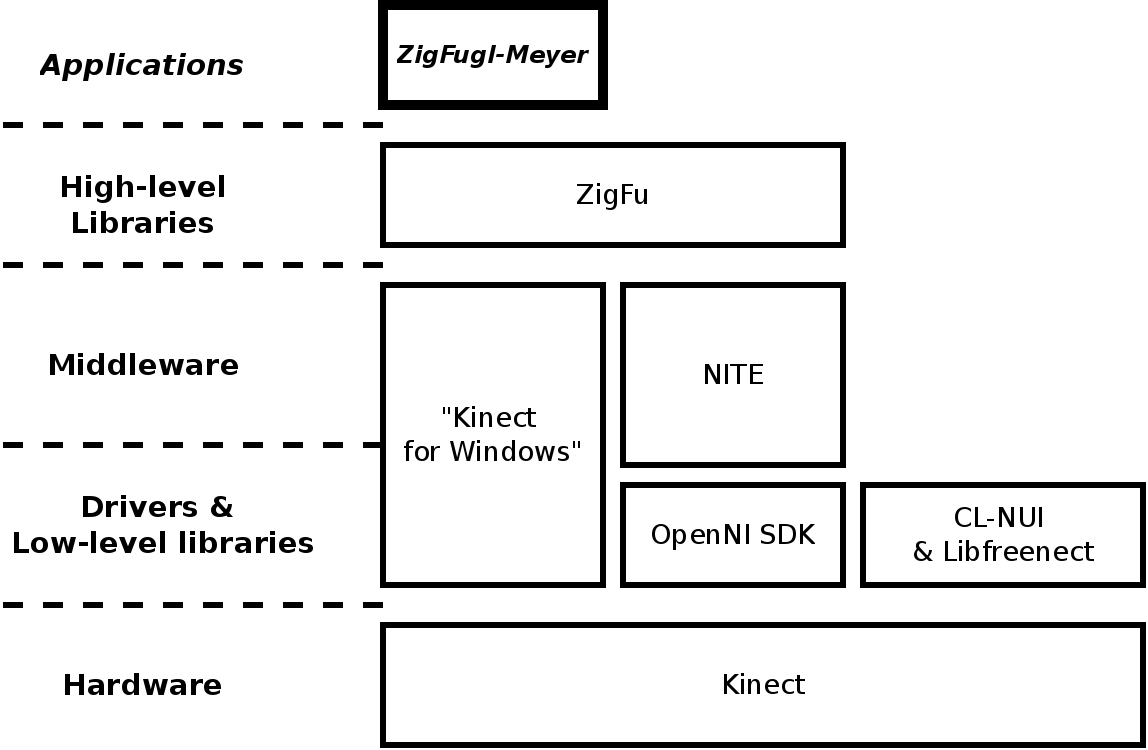
\includegraphics[width=0.9\linewidth]{../images/technology_overview_4}
\end{center}
\end{frame}

% ------------------------------------------------------------------------------
% PART III - MISE EN OEUVRE
% ------------------------------------------------------------------------------

%\section{Mise en \oe{}uvre}

\begin{frame}
\tableofcontents[currentsection, hideothersubsections]
\end{frame}

\subsection{Grapher}
\begin{frame}{Grapher}
\begin{center}
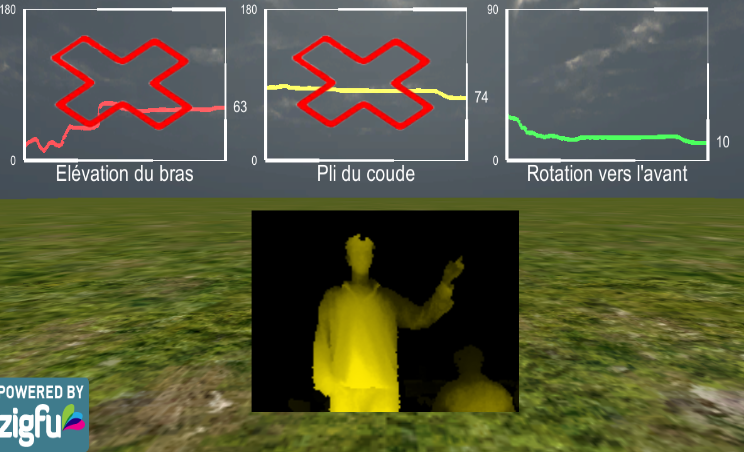
\includegraphics[width=0.9\linewidth]{../images/zfm_graph}
\end{center}
\end{frame}

\subsection{Multi Cameras}
\begin{frame}{Multi Cameras}
\begin{center}
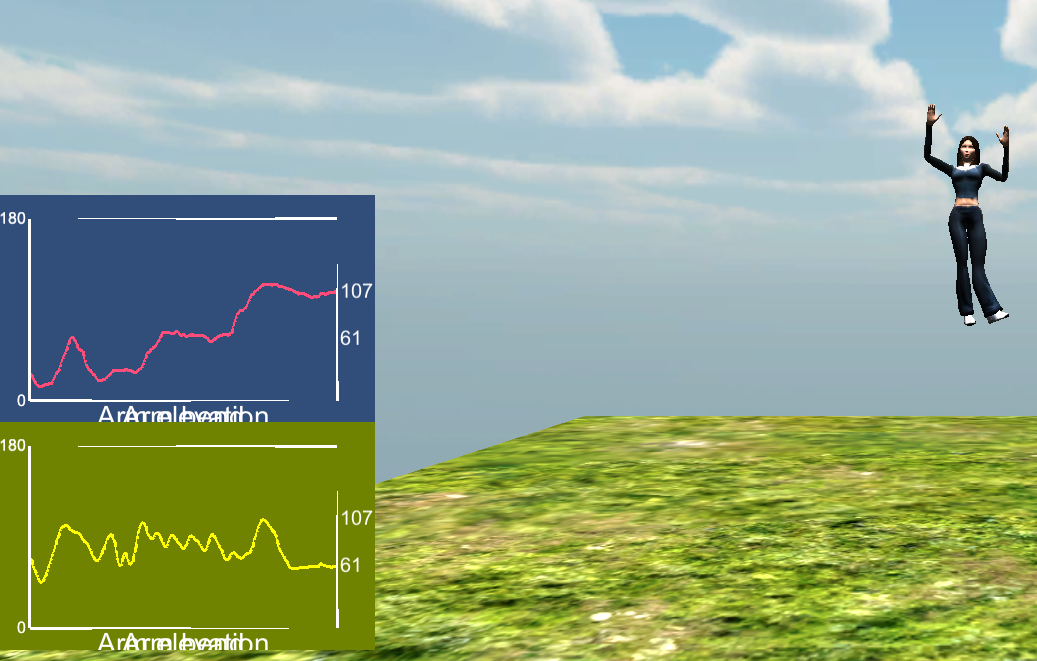
\includegraphics[width=0.9\linewidth]{../images/multicamera}
\end{center}
\end{frame}

\subsection{Avatar 3D}
\begin{frame}{Avatar 3D}
\begin{center}
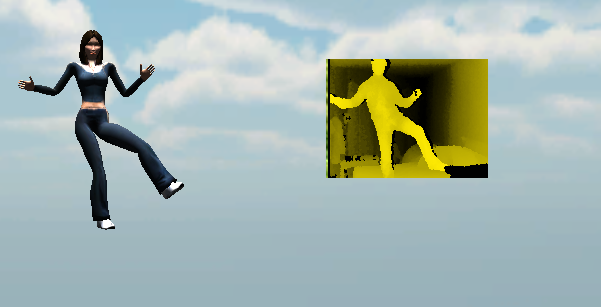
\includegraphics[width=0.9\linewidth]{../images/avatar3D}
\end{center}
\end{frame}

\subsection{Menus}
\begin{frame}{Menus}
\begin{center}
\only<1>{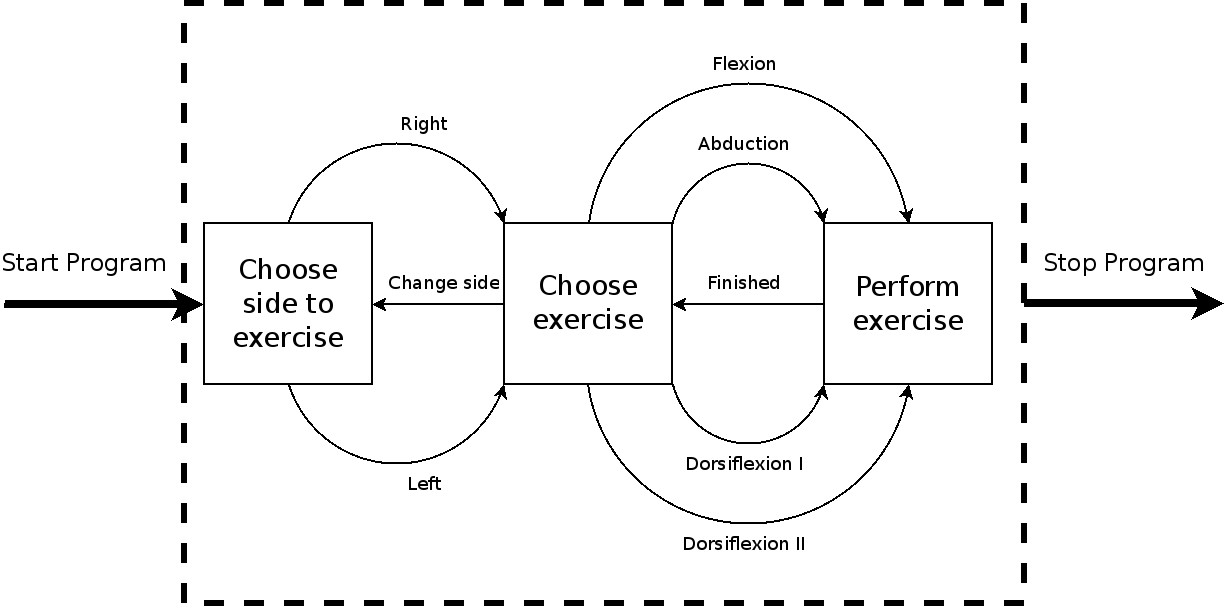
\includegraphics[width=1.0\linewidth]{../images/menu}}
\only<2>{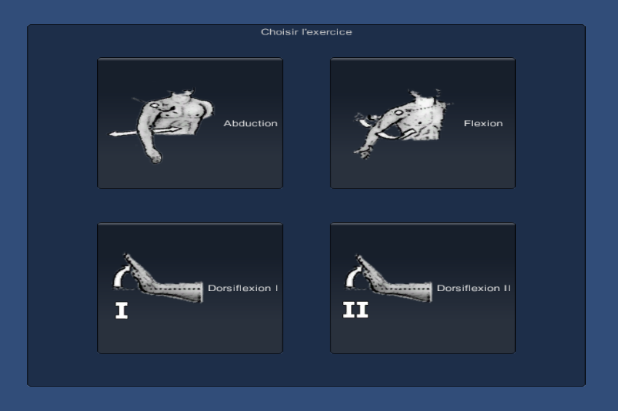
\includegraphics[width=0.8\linewidth]{../images/menu2}}
\end{center}
\end{frame}

\subsection{ExerciseMonitor}
\begin{frame}{Menus}
\begin{center}
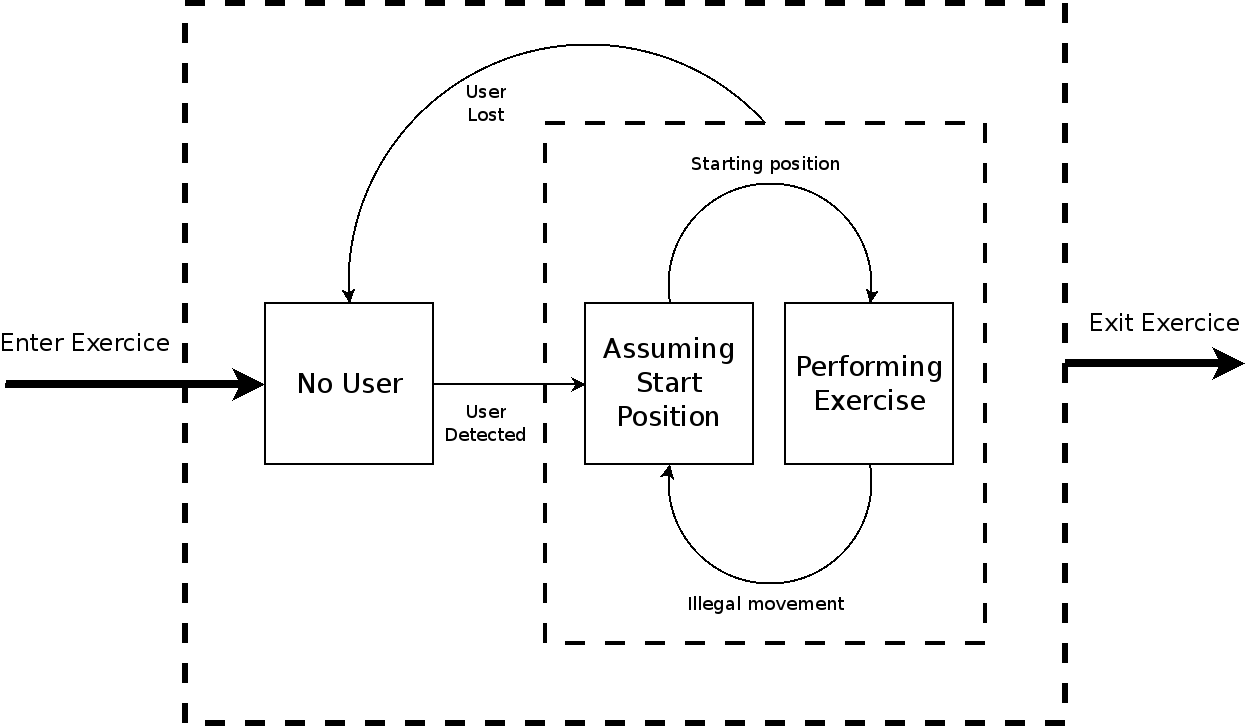
\includegraphics[width=1.0\linewidth]{../images/exercise_monitor}
\end{center}
\end{frame}

\subsection{À posteriori}
\begin{frame}{À posteriori}
\only<1-2>
{
  \begin{block}{Résultats}
  \begin{itemize}
  \item Test automatique,
  \item Retour granulaire,
  \item Aspect ludique qui émerge du retour d'informations.
  \end{itemize}
  \end{block}
}
\only<2>
{
  \begin{alertblock}{Problèmes}
  \begin{itemize}
  \item Trop de temps passé dans les menus,
  \item Le patient regarde le membre,
  \item Le retour incite à forcer.
  \end{itemize}
  \end{alertblock}
}
\only<3-4>
{
  \begin{alertblock}{Limites}
  \begin{itemize}
  \item Précision insuffisante,
  \item Pas de mesure des rotations,
  \item Zigfu.
  \end{itemize}
  \end{alertblock}
}
\only<4>
{
  \begin{block}{Ouverture}
  \begin{itemize}
  \item Poursuite de l'étude en stage~:
  \begin{itemize}
  \item \textbf{Geoffrey~:} aspects ludiques, difficulté dynamique,
  \item \textbf{William~:} meilleur extraction de squelette. 
  \end{itemize}
  \end{itemize}
  \end{block}
}

\end{frame}

% ------------------------------------------------------------------------------
% PART IV - CONCLUSIONS
% ------------------------------------------------------------------------------

\section{Conclusions}

\begin{frame}{Conclusions}
\only<1-2>
{
  \begin{block}{Résultats}
  \begin{itemize}
  \item Test automatique,
  \item Retour granulaire,
  \item Aspect ludique qui émerge du retour d'informations.
  \end{itemize}
  \end{block}
}
\only<2>
{
  \begin{alertblock}{Problèmes}
  \begin{itemize}
  \item Trop de temps passé dans les menus,
  \item Le patient regarde le membre,
  \item Le retour incite à forcer.
  \end{itemize}
  \end{alertblock}
}
\only<3-4>
{
  \begin{alertblock}{Limites}
  \begin{itemize}
  \item Précision insuffisante,
  \item Rotations déduites des positions,
  \item Zigfu.
  \end{itemize}
  \end{alertblock}
}
\only<4>
{
  \begin{block}{Ouverture}
  \begin{itemize}
  \item Poursuite de l'étude en stage~:
  \begin{itemize}
  \item \textbf{Geoffrey~:} paramétrage thérapeutique de jeu,
  \item \textbf{William~:} meilleur extraction de squelette. 
  \end{itemize}
  \end{itemize}
  \end{block}
}
\end{frame}

% ------------------------------------------------------------------------------
% PART V - DEMONSTRATION
% ------------------------------------------------------------------------------

\section{Démonstration}

\begin{frame}{trololo}
\end{frame}

% ------------------------------------------------------------------------------
% REFERENCES
% ------------------------------------------------------------------------------

\section{Références}
\begin{thebibliography}{200}
\makeatletter
    \clubpenalty10000
    \@clubpenalty \clubpenalty
    \widowpenalty10000
\makeatother

\begin{footnotesize}

\bibitem{newcombe2011}
  \emph{KinectFusion: Real-time dense surface mapping and tracking}
  \begin{tiny}
  Newcombe et al.\\
  Mixed and Augmented Reality (ISMAR), 2011 10th IEEE International Symposium on,
  \end{tiny}

\bibitem{izadi2011}
  \emph{KinectFusion: real-time 3D reconstruction and interaction using a moving depth camera}
  \begin{tiny}
  Izadi et al.\\
  Proceedings of the 24th annual ACM symposium on User interface software and technology,
  \url{http://doi.acm.org/10.1145/2047196.2047270}
  \end{tiny}
  
\bibitem{rules_of_play}
  \emph{Rules of Play: Game Design Fundamentals}\\
  \begin{tiny}
  Katie Salen, Eric Zimmerman,\\
  MIT Press (4 novembre 2003)
  \end{tiny}

\bibitem{flow}
  \emph{Flow (psychology) - page wikipedia}\\
  \begin{tiny}
  \url{http://en.wikipedia.org/wiki/Flow_\%28psychology\%29}
  \end{tiny}
  
\bibitem{ref_analyse_litterature}
  \emph{Evaluation of the disabilities of hemiplegic patients},\\
  \begin{tiny}
  Annuel de la médecine physique et de réadaptation, Juillet 2005,\\
  Gellez-Leman MC, Colle F, Bonan I, Bradai N, Yelnik A.\\
  \end{tiny}
  
\bibitem{leaps_fm}
  \emph{Fugl-Meyer Assessement of physical performance},\\
  \begin{tiny}
  Adapted from LEAPS (Locomotor Experience Applied Post-Stroke) manual,\\
  APTA Combined Sections meeting, 2008,\\
  \end{tiny}

\bibitem{atwiki_wiihab}
  \emph{Wii rehab applications (wiihab)}.\\
  \begin{tiny}
  \url{http://atwiki.assistivetech.net/index.php/Wii_rehab_applications_\%28wiihab\%29}
  \end{tiny}
  
\bibitem{homebrew_wii}
  \emph{List of development tools - Wii homebrew wiki}\\
  \begin{tiny}
  \url{http://wiibrew.org/wiki/List_of_development_tools}
  \end{tiny}
  
\bibitem{adafruit_bounty}
  \emph{The Open Kinect project - adafruit blog post}. \\
  \begin{tiny}
  \url{http://www.adafruit.com/blog/category/kinect-hacking/}\\
  \url{http://goo.gl/aSJTF} (lien raccourci)
  \end{tiny}

\bibitem{adafruit_winner}
  \emph{Open Kinect driver(s) released - adafruit blog post}\\
  \begin{tiny}
  \url{http://www.adafruit.com/blog/category/kinect-hacking/}\\
  \url{http://goo.gl/i49ki} (lien raccourci)
  \end{tiny}

\bibitem{clnui}
  \emph{CL NUI Platform}\\
  \begin{tiny}
  \url{http://codelaboratories.com/kb/nui}
  \end{tiny}
  
\bibitem{msdn_joint_orientation}
  \emph{MSDN - Kinect Joint Orientation}\\
  \begin{tiny}
  \url{http://msdn.microsoft.com/en-us/library/hh973073.aspx}
  \end{tiny}
  
\bibitem{microsoft_vs_openni}
  \emph{Kinect for Windows SDK Beta vs. OpenNI}\\
  \begin{tiny}
  Will Hinchman, 20 Juin 2012\\
  \url{http://labs.vectorform.com/2011/06/windows-kinect-sdk-vs-openni-2/}
  \end{tiny}
  
\bibitem{microsoft_vs_openni_2}
  \begin{tiny}
  Brekel, 18 Juin 2011\\
  \url{http://www.brekel.com/?p=677/}
  \end{tiny}
  
\bibitem{how_you_become_the_controller}
  \begin{tiny}
  Engineering Blog - xbox.com\\
  \url{http://123kinect.com/kinect-forums/thread-765.html}
  \url{http://www.xbox.com/en-US/Live/EngineeringBlog/122910-HowYouBecometheController}
  \end{tiny}

\bibitem{shotton2011}
  \begin{tiny}
  \emph{Real-Time Human Pose Recognition in Parts from Single Depth Images}\\
  Computer Vision and Pattern Recognition, Juin 2011\\
  \url{http://research.microsoft.com/apps/pubs/default.aspx?id=145347}
  \end{tiny}
  
\bibitem{openni_site}
  \emph{OpenNI - site web}\\
  \begin{tiny}
  \url{http://www.openni.org/}
  \end{tiny}
  
\bibitem{kinect_msdn}
  \emph{Kinect sur MSDN}\\
  \begin{tiny}
  \url{http://msdn.microsoft.com/en-us/library/jj131033.aspx}
  \url{http://msdn.microsoft.com/en-us/library/microsoft.kinect.colorimageformat.aspx}
  \url{http://msdn.microsoft.com/en-us/library/microsoft.kinect.depthimageformat.aspx}
  \end{tiny}

\bibitem{wiki_kinect}
  \emph{Kinect - page wikipedia}\\
  \begin{tiny}
  \url{http://en.wikipedia.org/wiki/Kinect}
  \end{tiny}
  
\bibitem{unity_docs}
  \emph{Documentation de Unity 3D}\\
  \begin{tiny}
  \url{http://docs.unity3d.com/}
  \end{tiny}
  
\bibitem{nightkit}
  \emph{Unity and Kinect tutorial - Nightmare Kitty}\\
  \begin{tiny}
  \url{http://www.nightmarekitty.com/2011/10/28/unity-and-kinect-tutorial/}
  \end{tiny}

\bibitem{zigfu_site}
  \emph{Zigfu - site web}\\
  \begin{tiny}
  \url{http://www.zigfu.com}
  \end{tiny}

\bibitem{zigfu_video}
  \emph{ZigFu at Microsoft VC Summit - vidéo Youtube}\\
  \begin{tiny}
  \url{http://www.youtube.com/watch?v=uSo0jXYm5wQ}
  \end{tiny}
  
\bibitem{zigfu_review}
  \emph{Microsoft Kinect and the web browser - enter Zigfu}\\
  \begin{tiny}
  Mairead, 1 Juin 2012\\
  \url{http://www.headlondon.com/our-thoughts/}\\
  \url{http://goo.gl/oTGdn} (lien raccourci)
  \end{tiny}
  
\bibitem{zigfu_branch}
  \emph{Projet UnityWrapper - github}\\
  \begin{tiny}
  \url{http://github.com/OpenNI/UnityWrapper}\\
  \url{http://github.com/tinkerer/UnityWrapper}
  \end{tiny}
  
\bibitem{mojos}
  \emph{MOJOS - site web}\\
  \begin{tiny}
  \url{http://www.mojos.fr/home/}
  \end{tiny}

\bibitem{creative_application}
  \emph{Creative Applications Network - site web}\\
  \begin{tiny}
  \url{http://www.creativeapplications.net}
  \url{http://www.creativeapplications.net/tutorials/guide-to-camera-types-for-interactive-installations/}
  \end{tiny}
  
\end{footnotesize}
\end{thebibliography}



\end{document}